\chapter{Controlador de corriente} \chapterlabel{Informe/4-ControladorCorriente} \label{cap:ControladorCorriente}

En este capítulo se diseña y modela el circuito encargado de controlar la corriente que circula por el electroimán. Como se vio en el capítulo anterior, el sistema trabaja con corrientes elevadas por lo que se implementan estrategias de conmutación para reducir las pérdidas de energía. Para ello se utiliza una topología de puente H con cuatro MOSFET y un \textsl{driver} que los controla. Además, se detallan los criterios tenidos en cuenta al momento de  elegir  y dimensionar todos los componentes que intervienen para lograr el correcto funcionamiento del controlador de corriente. Por último, se obtiene su función transferencia  para ser utilizada en el diseño del compensador.

\section{Descripción general}\label{sec_descripcion-general}

Para mantener en suspensión a la pieza móvil es necesario regular la fuerza electromagnética generada por el electroimán. Esto se logra modificando la intensidad de la corriente que circula por su bobinado como lo indica la expresión \ref{eq_fuerza_magnetica}. Por lo tanto, es necesario diseñar una fuente de alimentación que sea capaz de proveer la corriente requerida. 

Como se analizó en el capítulo \ref{cap:CaracterizacionElectroiman}, el electroimán puede ser modelado como una inductancia que varía con la distancia de entrehierro y una resistencia serie. Es decir, como un circuito RL serie cuya admitancia se muestra en la expresión \ref{eq_corriente}.

\begin{equation} \label{eq_corriente}
\frac{I_L}{V_L}(s)=\frac{1}{sL(Y_g)\ +\ R_L}
\end{equation}

Al aplicar la transformada inversa de Laplace a la expresión  \ref{eq_corriente}, se obtiene la respuesta temporal de la corriente ante un escalón de tensión con amplitud $v_L$ en la entrada, considerando corriente inicial $I_o$ y constante de tiempo $\tau=\frac{L(Y_g)}{R_L}$.

\begin{equation} \label{eq_corriente_temporal_cond_iniciales}
	i_L(t)=\frac{v_L}{R_L} + (I_o-\frac{v_L}{R_L})*e^{-\frac{t}{\tau}}
\end{equation}

En la expresión \ref{eq_corriente_temporal_cond_iniciales} se puede observar que la respuesta al escalón está compuesta por dos partes: un término con una exponencial negativa correspondiente al transitorio, y un término constante correspondiente al valor en régimen permanente $\frac{v_L}{R_L}$. El primero es el responsable de que la corriente en el inductor crezca de manera amortiguada, hasta alcanzar el valor de régimen permanente luego de cierto tiempo. Este comportamiento se puede observar en la simulación realizada en la figura \ref{fig:img_respuesta_escalon}. En la parte superior se observa la tensión de entrada y, en la inferior, la corriente del electroimán. Este análisis resulta de utilidad para conocer el comportamiento del electroimán y diseñar un controlador de corriente adecuado.


\begin{figure}[H]
	\centering
	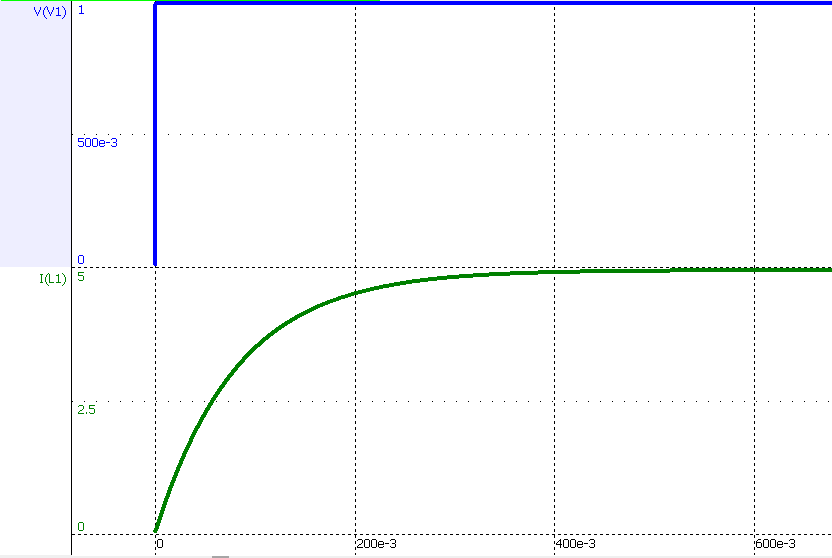
\includegraphics[scale=0.5]{corriente_escalon.png}
	\caption{Respuesta ante una entrada en escalón.}
	\label{fig:img_respuesta_escalon}
\end{figure}


\section{Diseño del controlador}

Se desea lograr controlar el valor medio de corriente que circula por el electroimán a partir de un sistema realimentado. Para ello se propone utilizar un controlador que trabaja en conmutación, alternando la alimentación del electroimán entre un valor superior positivo $\ V_{sup}$, y un valor inferior negativo $V_{inf}$. De esta manera, al controlar los tiempos de conmutación, se puede lograr una forma de onda como la que se muestra en la figura  \ref{fig:img_corriente_exponencial}. El resultado es que se obtiene una forma de onda oscilante cuyo valor medio $<I_L>$ es la corriente deseada. El resultado es una forma de onda con un valor medio correspondiente al deseado y un ripple superpuesto. La idea es que este ripple sea pequeño comparado con el valor medio, de manera que la planta pueda filtrarlo. 
